
\section{Experiment and demonstration}
\label{sec:live}

\begin{figure}
  \centering
  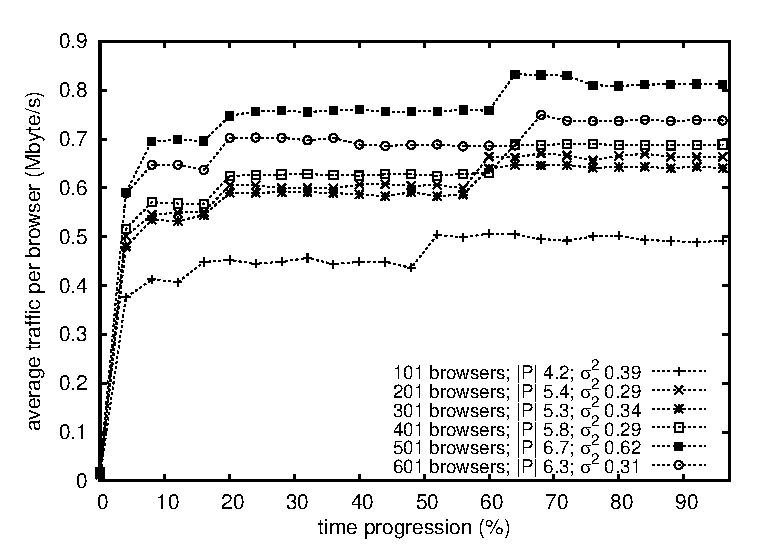
\includegraphics[width=0.49\textwidth]{img/traffic.eps}
  \caption{\label{fig:traffic}Average traffic per second.}
\end{figure}

In laboratory, we tested \CRATE on the Grid'5000 testbed with configurations
involving up till 600 browsers. Figure~\ref{fig:traffic} shows the traffic
generated at each member by intensive editing sessions. Overall, the artificial
authors insert 100 characters per second during 7 hours. The documents reach
millions of characters. Figure~\ref{fig:traffic} shows the combined effects of
\SPRAY and \LSEQ. Indeed, we observe that the traffic logarithmically scales to
the editing session size thanks to \SPRAY. The members of the smallest editing
session (101 browsers) are less traffic intensive than ones of the largest group
(601 browsers).  But the messages transiting the network are important too. The
growth of each plot corresponds to the identifiers size generated by
\LSEQ. Since the document size grows, the identifiers grow, but their growth
slows over insertions.


% \begin{figure*}
%   \centering
%   \subfloat[Figure A][\label{fig:liveA} Setup of the live
%   experiment. People start joining through a mediator server connected to our
%   replica. It incrementally builds an editing session with browsers
%   (cf. figure~\ref{fig:liveB}).]{
\begin{tikzpicture}[scale=1.1]
  
  \newcommand\X{30pt};
  \newcommand\Y{35pt};

  \draw[fill=white](0*\X, 0*\Y) node[align=center]{Mediator\\File server} +(-25pt,-10pt) rectangle +(25pt,10pt);
  \draw[fill=white](-2*\X, -2*\Y) node[align=center]{Our replica\\Measuring tools} +(-30pt,-10pt) rectangle +(30pt,10pt);

  \draw[fill=white](2*\X, -0*\Y)node{$s_1$} +(-5pt,-5pt) rectangle +(5pt,5pt);
  \draw[fill=white](4*\X, -0.5*\Y)node{$s_2$}  +(-5pt,-5pt) rectangle +(5pt,5pt);
  \draw[fill=white](3*\X, -1*\Y)node{$s_3$}  +(-5pt,-5pt) rectangle +(5pt,5pt);
  \draw[fill=white](2*\X, -2*\Y)node{$s_4$}  +(-5pt,-5pt) rectangle +(5pt,5pt);
  \draw[fill=white](4*\X, -2*\Y)node{$s_5$}  +(-5pt,-5pt) rectangle +(5pt,5pt);
  \draw[fill=white](3*\X, -2*\Y)node{$s_6$}  +(-5pt,-5pt) rectangle +(5pt,5pt);
  \draw[fill=white](1*\X, -2*\Y)node{$s_7$}  +(-5pt,-5pt) rectangle +(5pt,5pt);


  \draw[<->](0*\X, -10+0*\Y) -- (-2*\X, -2*\Y+10);
  \draw[<->, densely dashed] (0*\X+25,0*\Y) -- (2*\X-5, 0*\Y);
  
  \draw[<->, densely dashed] (0*\X+25,0*\Y-5) -- (4*\X-5, -0.5*\Y);
  \draw[<->, densely dashed] (0*\X+25,0*\Y-10) -- (3*\X-5, -1*\Y+5);
  \draw[<->, densely dashed] (0*\X+19,0*\Y-10) -- (4*\X-5, -2*\Y+5);
  \draw[<->, densely dashed] (0*\X+13,0*\Y-10) -- (3*\X-5, -2*\Y+5);
  \draw[<->, densely dashed] (0*\X+6,0*\Y-10) -- (2*\X-5, -2*\Y+5);
  \draw[<->, densely dashed] (0*\X+3,0*\Y-10) -- (1*\X-5, -2*\Y+5);

\end{tikzpicture}}
%   \hspace{10pt}
%   \subfloat[Figure B][\label{fig:liveB} Once connected, the editing session is
%   autonomous. The number of connections reflects the network size. Neigbhorhoods
%   are randomly filled and change over time.]{
\begin{tikzpicture}[scale=1]

  \newcommand\X{25pt}
  \newcommand\Y{-25pt}

  \draw[->] (\X, 0)--(\X, 5+3*\Y); %% p1 p6
  \draw[->] (-5+2*\X, 0)--(5+\X, 0); %% p2 p1
  \draw[->] (2*\X, 0) -- (-5+3*\X, \Y); %% p2 p3
  \draw[->] (2*\X, 0) -- (-5+3*\X, 2*\Y); %% p2 p4
  \draw[->] (3*\X, 5+\Y) -- ( 5+2*\X, 0); %% p3 p2
  \draw[->] (3*\X, \Y) -- (5pt, 2*\Y); %% p3 p7
  \draw[->] (3*\X, \Y) -- (2*\X, 5+3*\Y); %% p3 p5
  \draw[->] (3*\X, 2*\Y) -- (5pt, 2*\Y); %% p4 p7
  \draw[->] (3*\X, 2*\Y) -- (5pt, \Y); %% p4 p8
  \draw[->] (2*\X, 3*\Y) -- (\X, -5pt); %% p5 p1
  \draw[->] (5+2*\X, 3*\Y) -- (3*\X, -5+ 2*\Y); %% p5 p4
  \draw[->] (-5+\X, 3*\Y) -- (0pt, -5+2*\Y); %% p6 p7
  \draw[->] (0pt, 2*\Y) -- (-5+3*\X, \Y); %% p7 p3
  \draw[->] (0pt, 2*\Y) -- (\X, -5pt); %% p7 p1
  \draw[->] (0pt, \Y) -- (2*\X, -5pt); %% p8 p2
  \draw[->] (0pt, \Y) -- (\X, 5+3*\Y); %% p8 p6
  \draw[->] (0pt, \Y) -- (-5+3*\X, \Y); %% p8 p3
  
  \scriptsize
  \draw[fill=base3] (-2*\X, 1.5*\Y) node{$e_9$} +(-5pt,-5pt) rectangle +(5pt,5pt);
  \draw[<->, densely dashed, color=blue, thick] (-2*\X, 5+1.5*\Y) -- node[anchor=east]{join \ } (-2*\X, -5pt);

  \draw[fill=base3] (-2*\X, 0) node{$mediator_1$} +(-20pt, -5pt)rectangle+(20pt, 5pt);
  \draw[<->, densely dashed, color=red, thick] (20-2*\X, 0) -- node[anchor=south]{share} (-5+\X, 0);
  \draw[<->, densely dashed, color=red, thick] (20-2*\X, -5pt) -- (-5pt, \Y);
  
  \draw[fill=base3] (-2*\X, 3*\Y) node{$mediator_2$} +(-20pt, -5pt)rectangle+(20pt, 5pt);
  \draw[<->, densely dashed, color=red, thick] (20-2*\X, 3*\Y) -- (-5+\X, 3*\Y);
  \draw[<->, densely dashed, color=red, thick] (20-2*\X, 5+3*\Y) -- (-5pt, 2*\Y);

  \draw[fill=base3] (\X, 0)node{$e_1$}+(-5pt, -5pt)rectangle+(5pt, 5pt);
  \draw[fill=base3] (2*\X, 0)node{$e_2$}+(-5pt, -5pt)rectangle+(5pt, 5pt);
  \draw[fill=base3] (3*\X, \Y)node{$e_3$}+(-5pt, -5pt)rectangle+(5pt, 5pt);
  \draw[fill=base3] (3*\X, 2*\Y)node{$e_4$}+(-5pt, -5pt)rectangle+(5pt, 5pt);
  \draw[fill=base3] (2*\X, 3*\Y)node{$e_5$}+(-5pt, -5pt)rectangle+(5pt, 5pt);
  \draw[fill=base3] (1*\X, 3*\Y)node{$e_6$}+(-5pt, -5pt)rectangle+(5pt, 5pt);
  \draw[fill=base3] (0 , 2*\Y)node{$e_7$}+(-5pt, -5pt)rectangle+(5pt, 5pt);
%  \draw[fill=base3] (0 , \Y)+(-55pt, -10pt)rectangle+(5pt, 10pt);
  \draw[fill=base3](0,\Y) node{$e_8$}+(-5pt, -5pt)rectangle+(5pt, 5pt);

\end{tikzpicture}}
%   \caption{\label{fig:live} Live demo setup.}
% \end{figure*}

We would like to confirm the results of the experimentation by performing a live
demonstration of \CRATE that any WWW2016 participant can join. We will start an
\emph{exquisite
  corpse}\footnote{\url{https://en.wikipedia.org/wiki/Exquisite_corpse}}
collaborative storytelling. In this game, we will invite every participant to
continue or update the story initiated by previous participants.

In that regard, we will bootstrap an initial document in our local browser and
share it through a public URL advertised on twitter. Every participant will be
able to join the session by just clicking on this link. Next, she will freely
add a sentence. During the editing session, we will invite participant to share
and advertise the document with their friends in order to get as many
participants as possible.

During the experiment, we will be able to monitor the evolution of the document
and network. We expect the space complexity of the identifiers associated to
each character to be upper-bounded by $log(d)^2$ where $d$ is the number of
characters. We expect the partial view sizes to stay at $log(m)$ where $m$ is
the number of participants at a given time.
 
% Figure~\ref{fig:live} depicts the demonstration setup. Figure~\ref{fig:liveA}
% shows the joining process where people would open a link in their web browser
% which would give them access to the editing session kept alive by \emph{Our
%   replica}. Once a participant joins the editing session, it becomes part of a
% network of browsers the goal of which is to create a document. Our replica,
% still connected to the editing session would save the replica regularly and make
% measurements about:
% \begin{asparadesc}
% \item [\textbf{the replicated structure size:}] depending on how the document is
%   edited, the underlying sequence structure can grow heavily or remain balanced.
%   While papers often assume right-to-left editing, human behavior is less
%   predictable. Yet, we suppose that participants structure the document by
%   themself and because of the given context. Such editing behavior would lead to
%   a balanced data structure remaining efficient over time. 
% \item [\textbf{the network:}] the traffic generated by the editing session, its
%   number of participants, the average neighborhood tables size, the message rate
%   over time.
% \end{asparadesc}

% About the web application itself, we would like to collect anonymous opinions
% about:
% \begin{asparadesc}
% \item [\textbf{Functionality:}] were there enough functionnalities to complete
%   your task?
% \item [\textbf{Reliability:}] were there any trouble with the editor or the
%   network?
% \item [\textbf{Efficiency:}] did you feel that operations were not responding on
%   time?
% \item [\textbf{Communication:}] were you aware of other participants' changes?
% \end{asparadesc}


%% We also would like to collect opinions on software aspects through an
%% anonymous survey. (\TODO{cf paper www2012}).

%% 1 strongly disagree -> 4 neither agree nor disagree -> 7 strongly agree

%% Functionality (suitability)
%% %% Overall, the editor supported me completing the task in a collaborative way
%% Reliablity (Maturity, recoverability)
%% %% Synchronization did not hinder my work
%% %% Page reload hinder work
%% %% on error, i recover easily
%% %% how satisfied about recover speed
%% Usability (Learnability Operability Satisfaction)
%% %% easy to learn
%% %% easy to use
%% %% actions of other did not hinder my work
%% %% overall enjoyable
%% Efficiency (Efficiency compliance)
%% %% Reponsiveness of local
%% %% Responsiveness on remote
%% %% synchronization appealing
%% Communication (Information Gathering)
%% %% presence of other participant
%% %% recognize changes on document
%% %% action of other participant
%% %% appealing editor highlighting actions
%% Coordination (Shared Access)
%% %% easily start editing at any time
%% %% edit as long as desired
%% %% editor preserved the changes i made
%% %% easily start any tool any time
%% %% '' ''  use any tool as long as desired
%% %% appealing collbarative editing

%% \TODO{What do we do with data afterwards.}

%%% Local Variables:
%%% mode: latex
%%% TeX-master: "../paper"
%%% End:
